
 \chapter{Methods and fabrication.}

This Chapter outlines the methods used to fabricate the photonic circuits and quantum light source.
Once the components are fabricated and tested independently, they are bonded to form the Hybrid device.

\section{Waveguide fabrication and characterisation}

The SiON waveguide chip devices were fabricated by plasma enhanced chemical
vapour deposition to produce a layer of SiO$_2$ undercladding and SiON core on a
silicon substrate. Electron-beam lithography and reactive ion etching were used
to define the SiON core profile before finally an SiO$_2$ overclad layer was
defined. During the lithography process arbitrary waveguide shapes can be
imparted onto the device. These can be S-bends, directional couplers and/or Mach
Zehnder interferometers. Once the fabrication of the device was complete the
chips were then characterised. In this project the index of the core was 1.55
and the cladding was 1.51, the waveguide size was 1.6um to keep the guide single
mode. This is done to ensure that two photon interference can occur inside the
directional couplers.

\begin{figure}[h!] \begin{center}
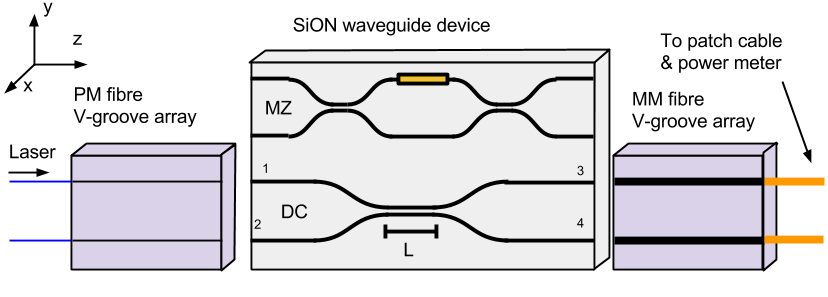
\includegraphics[width=0.8\textwidth]{images/wg_char.png} \end{center}
\caption{
Schematic of waveguide characterisation experiment. Two PM V-groove arrays are
aligned to the side  of the waveguide chip. One of the V-groove channels injects
laser light into port 1. The light is split by the DC and then collected from
port 3 and 4 by another (generally multimode) V-groove array and sent to a power
meter. The power ratios of of port 3 and 4 are used to calculate the coupling
ratio of the DC.
} \label{fig:6axis}
\end{figure}

Two V-groove arrays each were mounted on 6 axis stages which allowed precise
alignment of the V-grooves to the side of the SiON waveguide chip. The V-grooves
are commercially available arrays of fibres. A substrate is patterned with an
array of V shaped grooves into which optical fibres are planted and sealed, the polarisation axis
of the polarisation maintaining (PM) fibre is aligned to the vertical axis of the chip. This
experiment layout is shown in Figure \ref{fig:6axis}. One of the PM fibres
injects laser light into port 1. The laser used was a tuneable Fabry Perot
cavity laser emitting in the range 890 to 935nm. This light propagates through
the chip and is collected by the multimode V-groove array at ports 3 and 4 and
is then sent to power meters. This allows the calculation of the coupling ratio
of the directional couplers.

\subsection{Directional coupler ratio measurement}

Injecting light into port 1 and then 2 allows calculation of the coupling
ratio which is independent of the coupling loss. The coupling ratio in the
lossless case is as follows:

\begin{equation} r  = \frac{P_{13}}{I} = \frac{P_{24}}{I} \end{equation}

Where $P_{ij}$ is the power measured at port $j$ when light is injected into
port $i$. The parameter $I$ is the injected laser power. The conservation of
power in the lossless case allows:

\begin{equation} I = P_{13}+P_{14} = P_{23}+P_{24} \end{equation}

and

\begin{equation}\label{eqn:p1} P_{13}+P_{24} = Ir \end{equation}\label{eqn:p2}
\begin{equation} P_{14}+P_{23} = I(1-r) \end{equation}

However since there exists coupling loss and at each port, given by $l_i$, the
powers measured at each port become

\begin{equation} P^{'}_{ij} = l_i l_j P_{ij} \end{equation}

Then by taking a power ratio the losses can be canceled

\begin{equation} \frac{ P^{'}_{13} P^{'}_{24} }{ P^{'}_{14} P^{'}_{23} } =
\frac{ l_1 l_3 P_{13} l_2 l_4 P_{24} }{ l_1l_4P_{14}l_2l_3P_{23} }
\end{equation}

From Equation \ref{eqn:p1} and \ref{eqn:p2} this gives an expression for the
coupling ratio

\begin{equation} \left(\frac{r}{1-r}\right)*2 = \frac{P^{'}_{13}
P^{'}_{24}}{P^{'}_{14} P^{'}_{23}} \end{equation}

Rearranging to give

\begin{equation} r = \frac{\sqrt{\frac{P^{'}_{13} P^{'}_{24}}{P^{'}_{14}
P^{'}_{23}}}}{1+ \sqrt{\frac{P^{'}_{13} P^{'}_{24}}{P^{'}_{14} P^{'}_{23}}}}
\end{equation}

This allows an accurate calculation of the coupling ratio which is independent
of any coupling or alignment losses.

\subsection{Mach Zehnder interferometer visibility measurement}

In order to characterise the MZIs a very similar experiment was performed except
that the powers were recorded as a voltage was applied to the heater. Then the
effecive coupling ratio vs heater voltage was recorded. This shows how well the MZI can
switch light between the two ports, this is quantified by calculating the
visibility.

\begin{equation} V = 100 \frac{r_{max} - r_{min}}{r_{max} + r_{min}}
\end{equation}

This percentage shows the maximum switching capability of the MZI. A visibility
of 100\% means that all of the light can be coupled to one port, with no light
in the other. A visibility of 80\% means that, at best, the MZI will send only
80\% of the light to one port and 20\% to the other.

\section{Quantum dot growth and characterisation}

\subsection{Molecular beam epitaxy growth}

The QD source was grown by molecular beam epitaxy (MBE)\cite{cho1975molecular}.
MBE allows deposition of various semiconductor layers with atomic precision of
the layer height.

MBE take place in an ultra-high vacuum chamber, with pressures as low as
10$^{-8}$ Pa. A target wafer, in this case (110) oriented GaAs, is placed in the
chamber. The target materials, such as gallium and arsenic are placed in
separated crucibles, and heated until they begin to sublime. The gaseous
material will condense when it hits the wafer. If multiple elements hit the
wafer together they may react, for example a gallium arsenide layer may be
deposited.

\begin{figure}[h!] \begin{center}
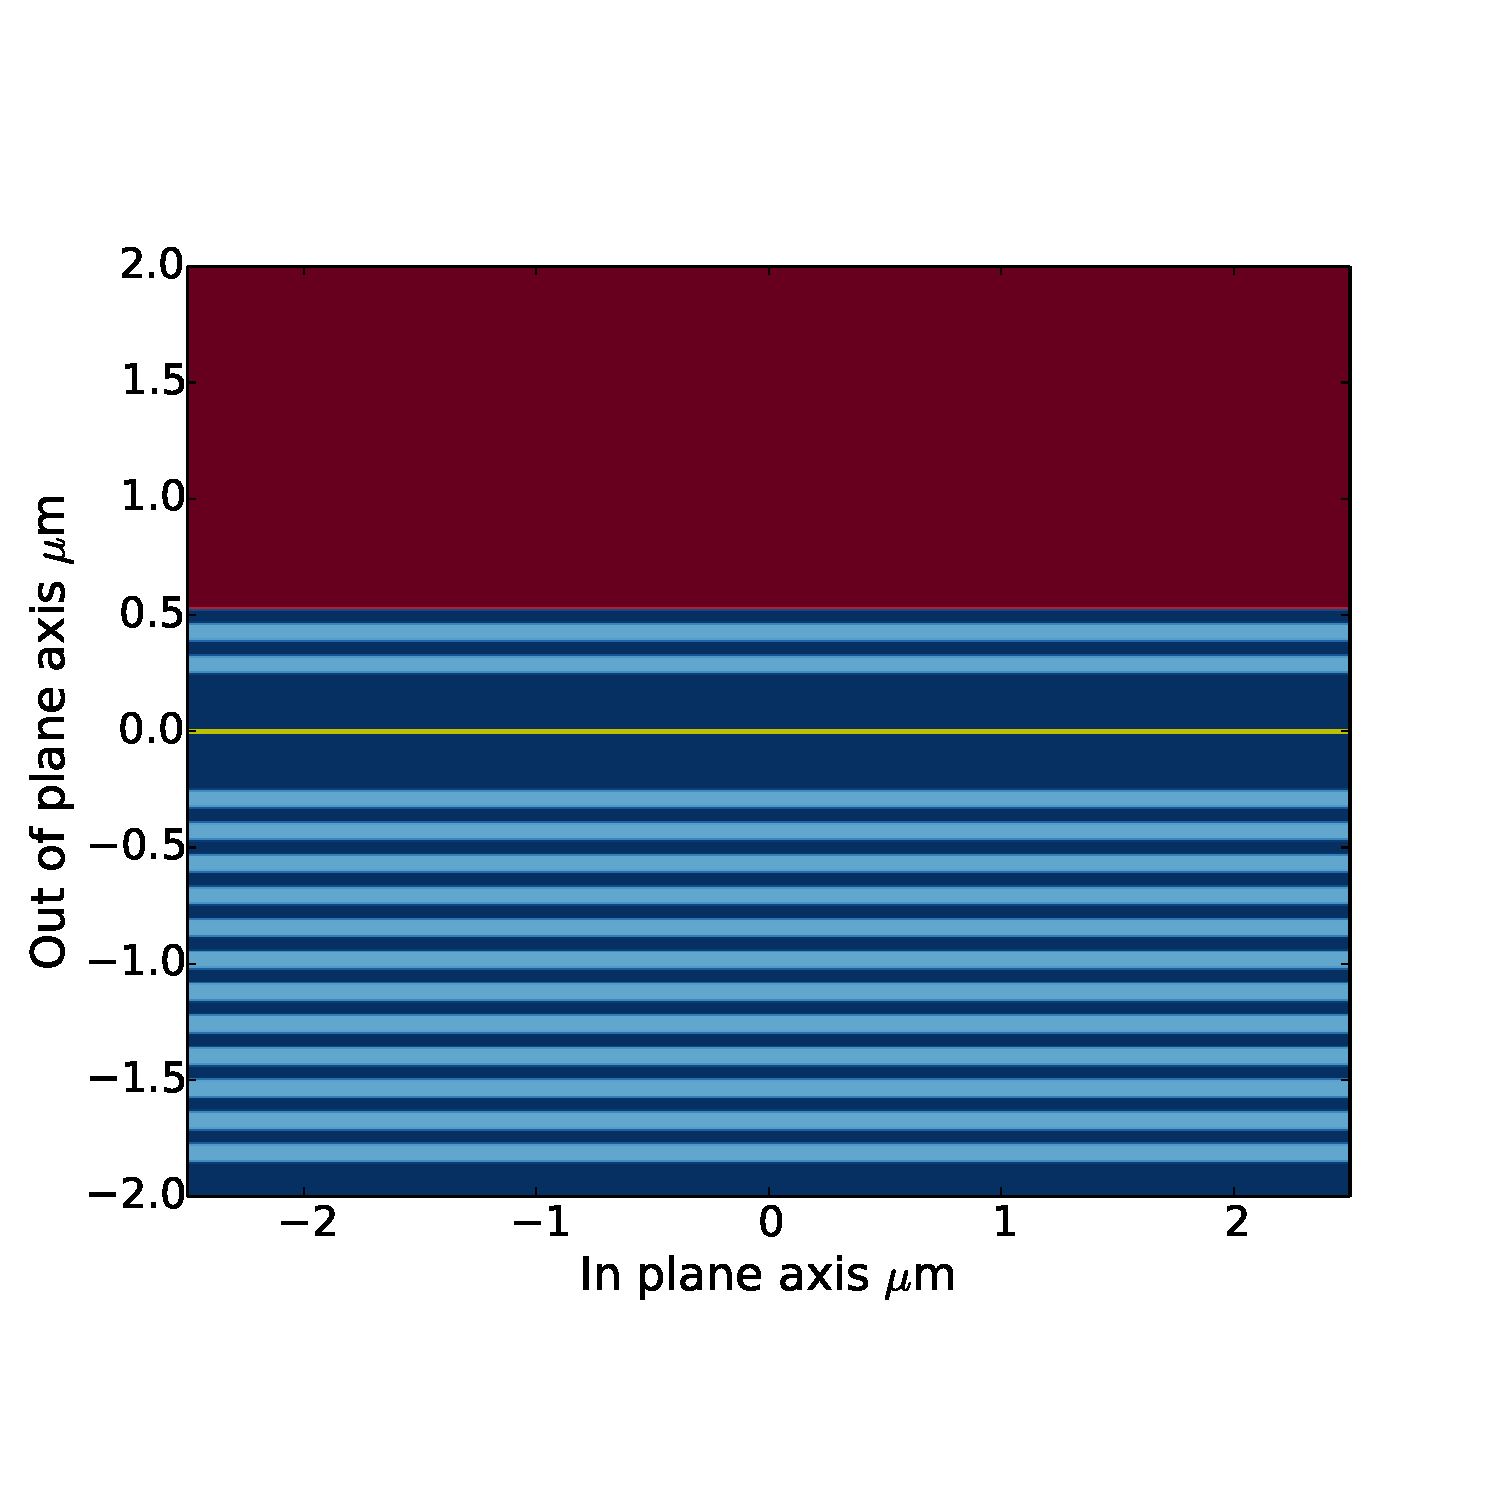
\includegraphics[width=0.75\textwidth]{images/qd_layers.pdf} \end{center}
\caption{
Index structure of the grown QD sample The red section is air with a
refractive index of 1 and the alternating blue layers are GaAs and AlAs.
}\label{fig:planar_cav} \end{figure}

By growing these layers carefully in Stranski–Krastanov mode InAs quantum dots
can be embedded into one of the layers. This layer is known as the wetting
layer, the size and composition of which dictate the QD
properties\cite{PhysRevB.70.125307}. Strain and chemical potential define a
critical layer thickness after which the growth of the layer will nucleate into
small semiconductor 'islands' \cite{PhysRevLett.64.1943}, inside which exist the
QDs.

The QD sample used in this project were embedded in a planar distributed bragg
reflector cavity to optimise the vertical emission mode from the
QDs\cite{bennett2005microcavity, 1367-2630-10-4-043035, Bennett_05}. The index
schematic of this structure is shown in Figure \ref{fig:planar_cav}. The
structure was grown on a GaAs substrate. Each reflector mirror repeat was made
by a layer of GaAs and a layer of AlAs. The cavity was created by placing twelve
mirror repeats of size $\lambda/4n$ where $\lambda = 910nm$ and $n$ is the
refractive index of the material. For GaAs this is 3.59 and for AlAs this is
2.97. Then a $2\lambda/n$ spacing of GaAs was grown with an embedded InAs layer
0.5nm thick. Finally two mirror repeats were grown on top. The emission
wavelength is typically in the range 890 to 950nm.

\subsection{Optical characterisation of quantum dots.}

\begin{figure}[h!] \begin{center}
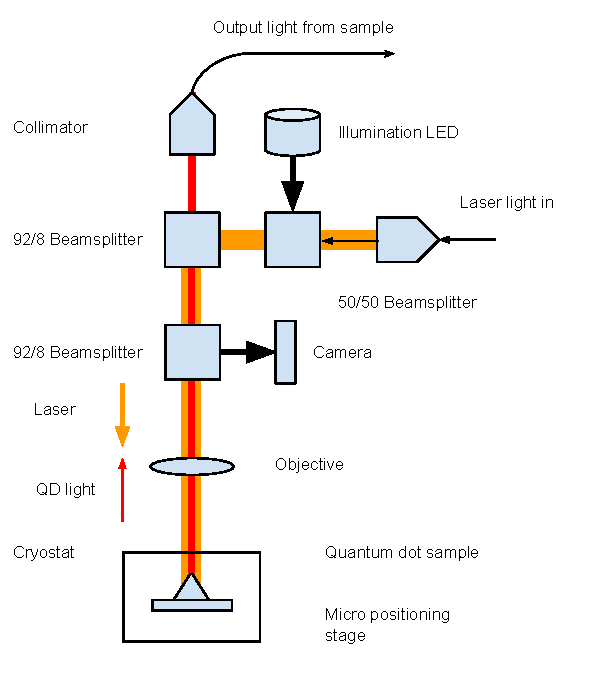
\includegraphics[width=0.5\textwidth]{images/qd_char.pdf} \caption{
Typical micro-Photoluminescence setup to excite the QD sample with a laser and
collect the QD light. The orange light is the laser and the red light is the
path the QD light takes. The QD light travels in free space through two 92/8
beamsplitters, with 92\% transmission. With the two beamsplitters, the laser,
LED and CCD elements can be placed in the optical path of the QD light, while
minimising the amount of QD light lost. The QD light is collected by a  fibre
coupled collimator and sent to a silicon charged coupled device (liquid nitrogen
cooled) equipped spectrometer.

} \label{fig:qd_char} \end{center} \end{figure}

To characterise a QD source it is first placed in a cryostat and measured in the
typical micro-Photoluminescence setup, shown in Figure \ref{fig:qd_char}. The
setup was mounted on  a 3-axis micrometer resolution stage in order to check
different areas of the sample under test.

The source is mounted in a continuous Helium flow cryostat. The sample is kept
below 10K for the duration of the experiments.

An LED is used to illuminate the sample, and a CCD camera allows realtime
imaging of the position of the sample. The LED is red and is turned off during
experiments so as not to excite the sample.

Above band laser excitation is used to excite the states in the sample. The
fibre-coupled laser light is collimated and then sent in free space to the
sample, through an infinity corrected objective lens. The objective normally
offers 50x or 100x magnification.

The light from the sample is then sent in free space through two 92/8
beamsplitters, with 92\% transmission. This is done so that the laser, LED and
CCD elements can be placed in the optical path of the sample light, but that the
minimum amount of sample light is lost.

The sample light is fibre coupled via collimator and sent to a silicon
charged coupled device (liquid nitrogen cooled) equipped spectrometer.

\subsection{Hanbury-Brown and Twiss measurements}

\begin{figure}[h!] \begin{center}
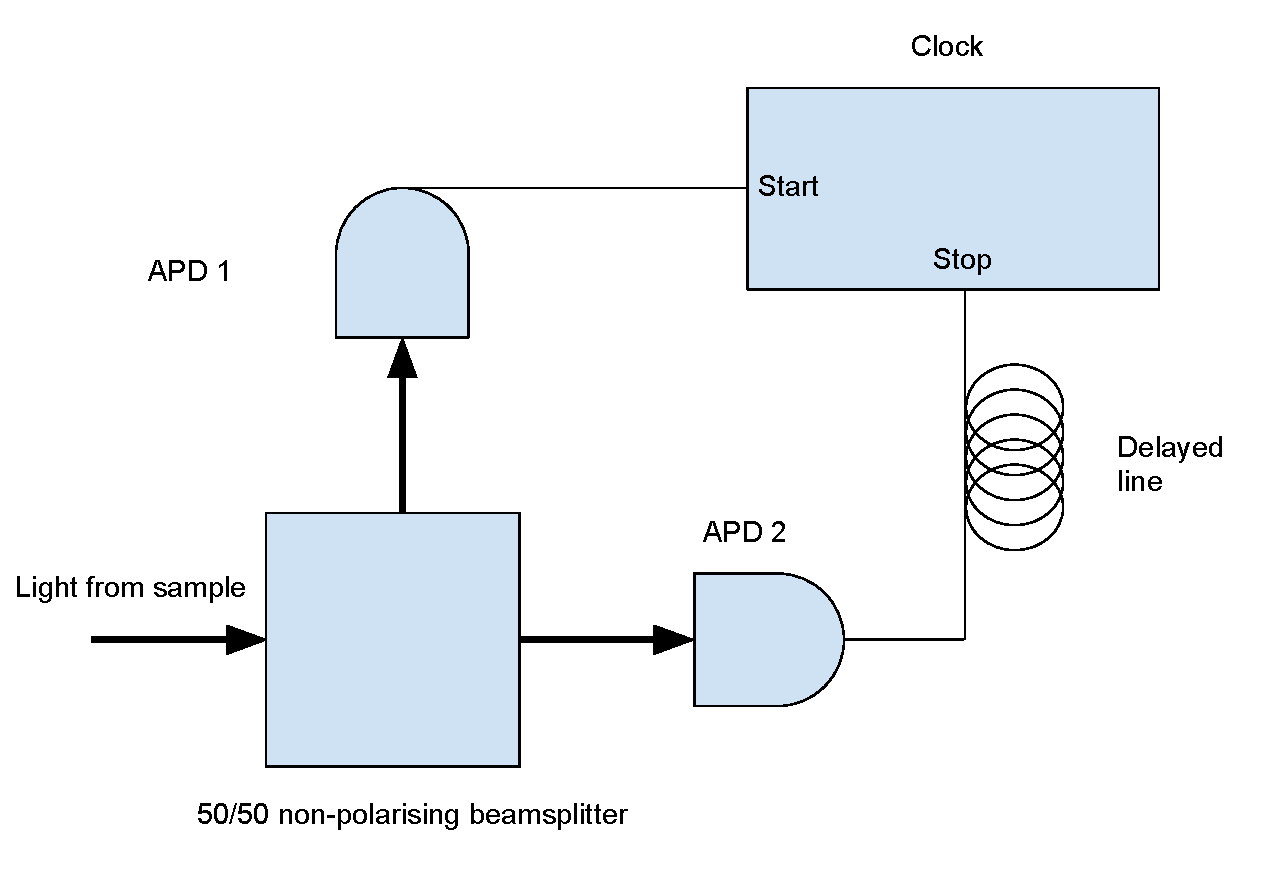
\includegraphics[width=0.7\textwidth]{images/basic_hbt.pdf} \caption{ Typical
HBT experiment, a stream of photons is sent to a balanced non-polarising
beamsplitter. The split beam is then sent to two APDs whose signals are
timestamped and correlated by a clock. The stop APD has a delay line in order to
achieve negative correlation values. } \label{fig:basic_hbt} \end{center}
\end{figure}

To verify the single photon nature of the QD emission a Hanbury Brown and Twiss
experiment must be performed. The second order correlation function
$g^{(2)}(\tau)$, as explained in Chapter 1, is measured by splitting a stream of
photons by a DC or beamsplitter. This experiment is shown schematically in
Figure \ref{fig:basic_hbt}.  Both streams are then sent to avalanche photodiodes
(APDs) where the arrival time of each photon is measured. One APD starts a clock
and the other stops it. By correlating the detection times of both APDs a correlation
histogram is built up. One APD is delayed by some time $\tau$ in order to
measure negative correlation values. An absence of counts at time $\tau = 0$
implies single photon emission.

\section{Hybrid device}

\begin{figure}[h!] \begin{center}
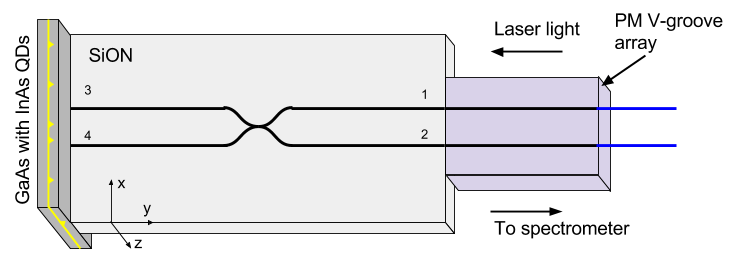
\includegraphics[width=1\textwidth]{images/hyb_basic.png} \caption{
Schematic of a hybrid device. A III-V chip with embedded quantum dots is bonded
to an SiON waveguide chip such that the single photons from the QDs are routed
through the waveguides. The other end of the waveguide is bonded to a V-groove
array to collect the light and send it to a spectrometer.
} \label{fig:hyb_basic} \end{center} \end{figure}

The III-V chip was bonded orthogonally to the SiON waveguide chip as shown in
Figure \ref{fig:hyb_basic} by UV cured adhesive. This allows the surface
emission of the III-V chip to be collected by the waveguides. The DC is needed
to allow separate fibres to be used for laser delivery and for QD light collection. The
laser light is delivered through port 1. The laser power is split by the DC and
will excite QDs at the ends of ports 3 and 4. This QD is collected by the
waveguides and will be split by the DC and sent to ports 1 and 2. That which
reaches port 2 is sent to the spectrometer. Typically the first experiment
performed on a new device is to check the spectrum and  to try and isolate a
single QD, exhibited by a narrow well defined peak. Throughout this project the
laser used was above the bandgap of GaAs, resonant or quasi-resonant excitation
was not used. The device shown in Figure \ref{fig:hyb_basic} is useful only to
check the emission of the QD into the waveguide, no on-chip quantum operations
can take place because all the available waveguides are used for excitation and
collection. In the next chapter a more sophisticated device with an on-chip MZI
will be discussed.

\subsection{Characterisation of quantum dots in hybrid circuit.}

\begin{figure}[h!] \begin{center}
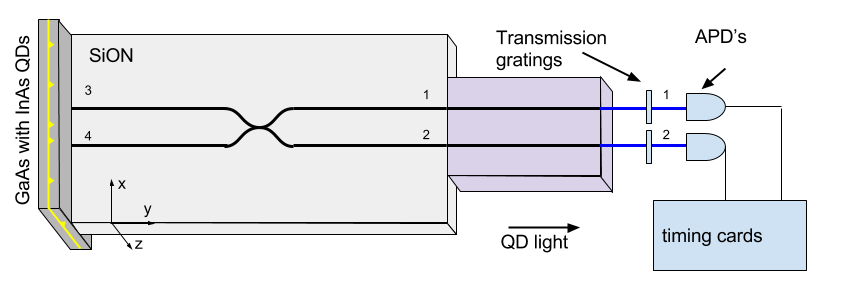
\includegraphics[width=1\textwidth]{images/hyb_hbt.png} \caption{
Schematic of HBT experiment taking place on the Hybrid chip. The light from
ports 1 and 2 of the hybrid chip is collected by the V-groove array and sent
towards transmission gratings in order to spectrally isolate the QD light.  The
light in both channels then impinge on APDs. The APD clicks are then correlated
on a timeing card.
} \label{fig:hyb_basic_hbt}\end{center} \end{figure}

In the case of the integrated hybrid chip, the HBT experiment, schematically shown in Figure
\ref{fig:hyb_basic_hbt}, the beamsplitting takes plane using the directional
coupler on-chip. But instead of sending the QD light from ports 1 and 2 to a
spectrometer it is sent towards two monochromators. This is so that only the
light from the target QD can be send towards the APDs and not background light,
or light from other QDs.

Doing the experiment on-chip offers greater long term stability than a typical non-integrated QD
experiment. In typical non-integrated HBT elaborate stability feedback loops
need to implemented in order to keep the QD APD counts constant long enough to
get a statistically significant result.
